\chapter{Contexte general du projet :}
\section{Presentation du centre :}
Le Code 212 est un centre de formation et de certification dans les metiers du digital, lance dans le cadre du Plan d'Acceleration de la Croissance et de la Transformation de l'economie (PACTE) ESRI-2030 au Maroc. Ce programme vise à repondre aux enjeux actuels et futurs lies à l'emergence des technologies numeriques en offrant des filières specifiques et des formations certifiantes. L'objectif est de renforcer les competences et les qualifications dans le secteur numerique, contribuant ainsi à l'atteinte des objectifs de developpement du pays, notamment celui de faire passer la part du secteur numerique à 5% du PIB d'ici 2035.

Le principal objectif du Centre Code 212 est de former une nouvelle generation de professionnels qualifies dans le domaine du numerique afin de repondre aux besoins croissants du marche de l'emploi dans ce secteur en plein essor. En offrant des formations specialisees et des certifications reconnues, le centre vise à fournir aux apprenants les competences et les connaissances necessaires pour reussir dans des domaines tels que le developpement web, la cybersecurite, l'analyse de donnees, le marketing digital et bien d'autres. En outre, le centre s'engage à promouvoir l'innovation et l'entrepreneuriat en encourageant les initiatives creatives et en offrant un environnement propice à l'emergence de projets novateurs dans le domaine du digital.

\subsection{Fiche du centre Code 212}

\begin{tabular}{|l|l|}
\hline
\textbf{Nom du Centre} & Code 212 \\
\hline
\textbf{Domaine d'Activite} & Formation et certification dans les metiers du digital \\
\hline
\textbf{Programme} & Plan d'Acceleration de la Croissance et de la Transformation de l'economie (PACTE) ESRI-2030 \\
\hline
\textbf{Localisation} & Maroc \\
\hline
\textbf{Objectif} & Renforcer les competences et les qualifications dans le secteur numerique \\
\hline
\textbf{Contributions} & Atteindre 5\% du PIB du secteur numerique d'ici 2035 \\
\hline
\textbf{Domaines de Formation} & 
\begin{tabular}{@{}l@{}}
- Developpement web \\
- Cybersecurite \\
- Analyse de donnees \\
- Marketing digital \\
- et bien d'autres
\end{tabular} \\
\hline
\textbf{Engagement} & 
\begin{tabular}{@{}l@{}}
- Promouvoir l'innovation \\
- Encourager l'entrepreneuriat \\
- Offrir un environnement propice aux projets novateurs
\end{tabular} \\
\hline
\end{tabular}


\subsection{Centre Code212}
\begin{figure}[H]
\centering
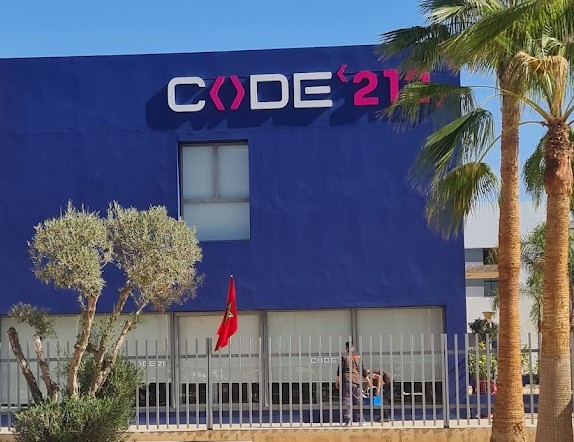
\includegraphics[height=10cm , width=\textwidth]{assets/images/code.jpg}
\caption{Centre Code 212 Agadir}
\label{fig:imagecentre}
\end{figure}

\begin{figure}[H]
\centering
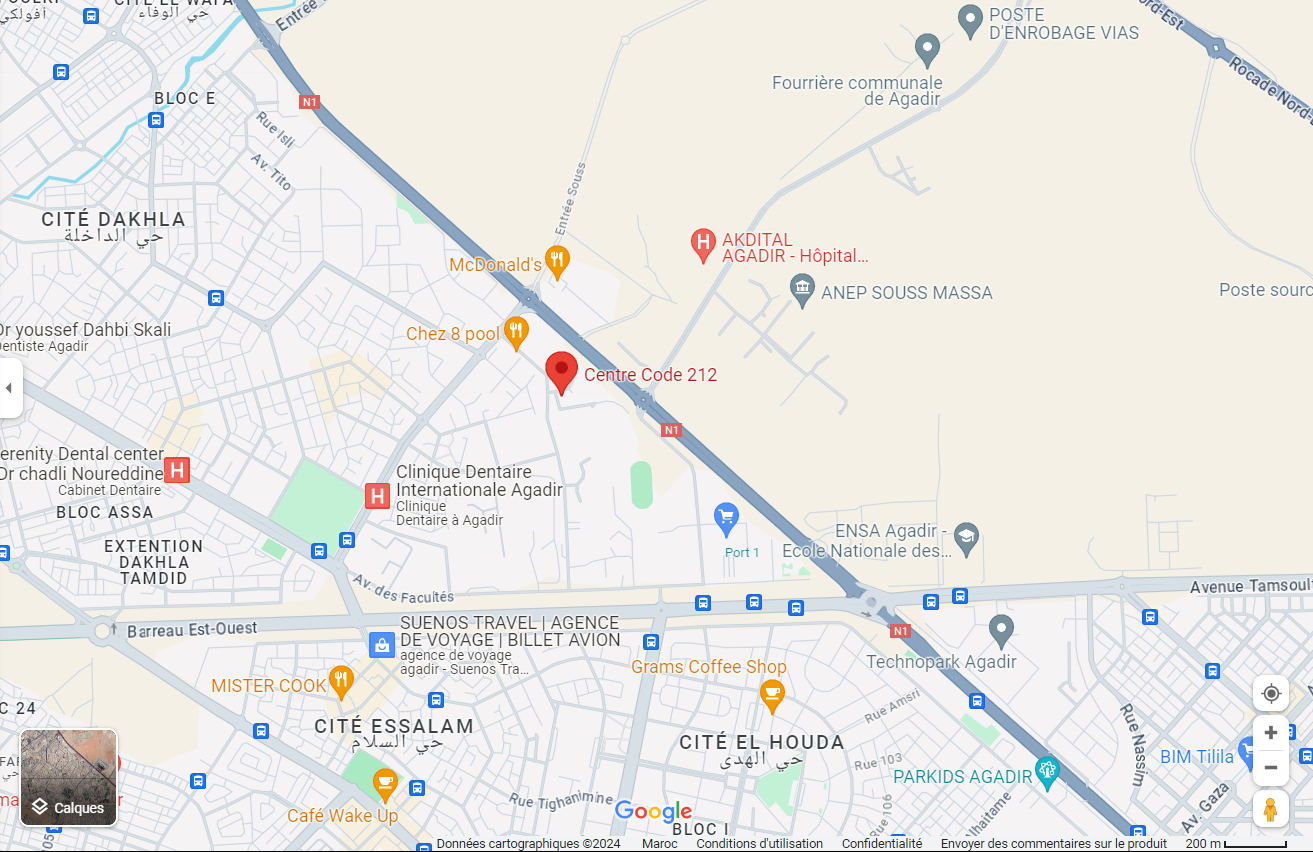
\includegraphics[height=10cm , width=\textwidth]{assets/images/maps.png}
\caption{Localisation du centre}
\label{fig:localisationcentre}
\end{figure}

\subsection{Domaine d'activites :}

\subsubsection{education et Pedagogie :}
L'education et la pedagogie au sein des centres Code 212 se focalisent sur la fourniture d'une formation specialisee en codage et programmation informatique, adoptant une methode d'enseignement innovante basee sur le peer-to-peer. Cette approche encourage les etudiants à apprendre les uns des autres dans un cadre collaboratif, sans dependance à un enseignement centralise traditionnel, favorisant ainsi l'autonomie et le developpement de competences pratiques en resolution de problèmes. Avec l'ouverture de ces centres, telle celle à l'Universite Ibn Zohr d'Agadir, les etudiants auront accès à une education de pointe en technologie, preparant la nouvelle generation à relever les defis de l'ère numerique et à contribuer activement au marche du travail dans le domaine de l'informatique.

\subsubsection{Renforcement des competences et employabilite :}
Code 212 est dedie à renforcer les competences digitales des etudiants marocains, favorisant ainsi leur employabilite dans un marche en pleine digitalisation. Grâce à des plateformes d'apprentissage interactives et des simulateurs d'examens, les etudiants pratiquent et valident leurs connaissances dans des conditions realistes, les preparant à repondre aux exigences des emplois actuels. Le centre s'engage à tracer un chemin clair pour ses etudiants vers des carrières numeriques florissantes, en leur donnant les outils pour innover et exceller dans une economie de plus en plus axee sur les technologies numeriques.
